\section{ORM}
El mapeo de objeto-relación (Object-Relational Mapping) es es un modelo de programación que convierte las tablas de una base de datos en entidades que faciliten el acceso a los datos a los programadores.
Las herramientas ORM evitan que los programadores tengan que aplicar consultas complejas en lenguaje SQL, al aplicar una capa de abstracción sobre la base de datos se agiliza el desarrollo y se puede escribir código con una legibilidad mayor.
Los ORM también aportan herramientas como la validación de datos, generación de estructuras, protección contra ataques SQL, definición de relaciones, entre otras.

El proceso de transformación utilizado por un ORM se describe en el siguiente diagrama:

\begin{figure}[H]
  \begin{center}
    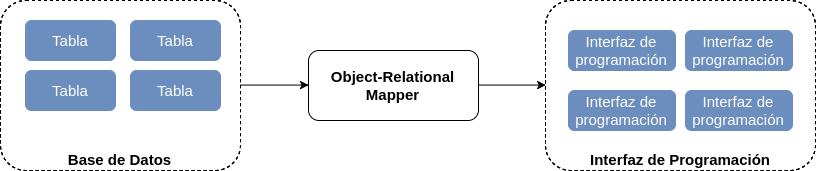
\includegraphics[scale= 0.5]{ORMArch}
  \end{center}
  \caption{Proceso de mapeo de un ORM}
\end{figure}

\section{Hibernate}
Hibernate es un framework ORM, que, además de contar con su propia API nativa, también es una implementación de la JPA (Java Persistence API), por lo que es posible integrarla con aplicaciones Java SE, Java EE, y otras tecnologías relacionadas.
Hibernate es conocido por su alto desempeño, escalabilidad, estabilidad y calidad, lo que hace de este ORM la opción por excelencia a la hora de desarrollar aplicaciones Java. 
